%       File: to_publish.Rnw
%       Author: Michael Quinn
%       Date Created: February 4, 2014
%       
%       Summary:
%                   This rnw is for a paper submitted to the Central Asia Business Journal.
%                   It is a self-contained document and downloads all needed data from the internet
%                   See abstract for more information
%%%%%%%%%%%%%%%%%%%%%%%%%%%%%%%%%%%%%%%%%%

% !Rnw weave = knitr

\documentclass[a4paper]{article}\usepackage[]{graphicx}\usepackage[]{color}
%% maxwidth is the original width if it is less than linewidth
%% otherwise use linewidth (to make sure the graphics do not exceed the margin)
\makeatletter
\def\maxwidth{ %
  \ifdim\Gin@nat@width>\linewidth
    \linewidth
  \else
    \Gin@nat@width
  \fi
}
\makeatother

\definecolor{fgcolor}{rgb}{0.345, 0.345, 0.345}
\newcommand{\hlnum}[1]{\textcolor[rgb]{0.686,0.059,0.569}{#1}}%
\newcommand{\hlstr}[1]{\textcolor[rgb]{0.192,0.494,0.8}{#1}}%
\newcommand{\hlcom}[1]{\textcolor[rgb]{0.678,0.584,0.686}{\textit{#1}}}%
\newcommand{\hlopt}[1]{\textcolor[rgb]{0,0,0}{#1}}%
\newcommand{\hlstd}[1]{\textcolor[rgb]{0.345,0.345,0.345}{#1}}%
\newcommand{\hlkwa}[1]{\textcolor[rgb]{0.161,0.373,0.58}{\textbf{#1}}}%
\newcommand{\hlkwb}[1]{\textcolor[rgb]{0.69,0.353,0.396}{#1}}%
\newcommand{\hlkwc}[1]{\textcolor[rgb]{0.333,0.667,0.333}{#1}}%
\newcommand{\hlkwd}[1]{\textcolor[rgb]{0.737,0.353,0.396}{\textbf{#1}}}%

\usepackage{framed}
\makeatletter
\newenvironment{kframe}{%
 \def\at@end@of@kframe{}%
 \ifinner\ifhmode%
  \def\at@end@of@kframe{\end{minipage}}%
  \begin{minipage}{\columnwidth}%
 \fi\fi%
 \def\FrameCommand##1{\hskip\@totalleftmargin \hskip-\fboxsep
 \colorbox{shadecolor}{##1}\hskip-\fboxsep
     % There is no \\@totalrightmargin, so:
     \hskip-\linewidth \hskip-\@totalleftmargin \hskip\columnwidth}%
 \MakeFramed {\advance\hsize-\width
   \@totalleftmargin\z@ \linewidth\hsize
   \@setminipage}}%
 {\par\unskip\endMakeFramed%
 \at@end@of@kframe}
\makeatother

\definecolor{shadecolor}{rgb}{.97, .97, .97}
\definecolor{messagecolor}{rgb}{0, 0, 0}
\definecolor{warningcolor}{rgb}{1, 0, 1}
\definecolor{errorcolor}{rgb}{1, 0, 0}
\newenvironment{knitrout}{}{} % an empty environment to be redefined in TeX

\usepackage{alltt}

\usepackage{graphicx} % For eps figures
\usepackage{graphics}
\usepackage{hyperref} % For urls
\usepackage{float} % Set exact location of figures
\usepackage{amsmath} % More elements for more complicated equations
\usepackage{amstext} % defines the \text command
\usepackage{amssymb}   % More statistics tools
\usepackage{amsthm}   % For proofs
\usepackage[numbib,notlof,notlot,nottoc]{tocbibind} % Section number for references
\usepackage{array,multirow} % for advanced column specification: use >{\command} for
                        % commands executed right before each column element
                        % and <{\command} for commands to be executed right after
                        % each column element

\usepackage{subfig}                                          % Fix the captions
\captionsetup[table]{aboveskip=6pt}

\title{Bayesian Estimates of the Parameters for Portfolio Optimization}
\date{\today}
\author{Michael Quinn \\ The University of Illinois at Urbana-Champaign\footnote{A project repository is available on Github. This includes the original .Rnw file for generating this paper and supplementary \texttt{R} code used in this project. See here: \url{https://github.com/michaelquinn32/Bayesian_Pricing_Paper.}}}
\IfFileExists{upquote.sty}{\usepackage{upquote}}{}
\begin{document}




\maketitle

\begin{abstract}
Bayesian estimation techniques are proposed to find the parameters for a minimum variance portfolio within the Markowitz framework. Motivation for this method comes from a series of scenarios relating to an analyst's confidence in the generalizability of  very recent stock data. The paper posits that an optimal stock allocation relies on a balance between recent and long-term stock behavior. The usage of prior distributions for the parameters allows for this balance. Monte Carlo sampling techniques are used to validate results.
\end{abstract}

\section{Introduction}

Most of contemporary financial theory traces its lineage back to Harry Markowitz (1952) \cite{mark52} and a solution to a very specific optimization problem: given a selection of multiple assets, what's the best way to make a portfolio? There are nearly countless answers to this question, each depending on their own assumptions about ways in which investors try to maximize personal utility. Investors could, for example, seek to maximize long-term wealth, or, just as easily, they could seek to maximize immediate gain. Either perspective depends on the investor's personal attitude towards risk.

Markowitz's model does not try to answer any questions about personal preferences about risk. All investors are different, and all will have different reasons for preferring different risk levels. Instead, Markowitz assumes general \textit{risk aversion}. That is, given a certain attitude towards risk, any investor will prefer to maximize their return without increasing the risk of this return. This is the same as saying that an investor will seek to minimize the risk of attaining any level of return on their investment.

How can they do this? The answer is surprisingly simple: diversify. A broad basket of returns will minimize the risk of any one asset under-performing, allowing for a reduction in risk. Similarly, given the choice of a wide variety of assets and the option to borrow or lend at a risk free rate, any investor is capable of forming a portfolio that maximizes their possible return at a given risk level. Markowitz named this the \textit{efficient portfolio frontier}.

Markowitz's model is not without its criticisms. For the purposes of this paper, we will focus on three:

\begin{itemize}
    \item The outputs of the Markowitz model are very sensitize to input parameters (Best and Grauer, 1991) \cite{best91}. This is especially true for expected returns.
    \item Stock data is often very noisy, which leads to a high chance for estimation error (Chopra and Ziemba, 1993) \cite{chopra93}. Considering that asset fundamentals are dynamic, an analyst is challenged to balance relevant and representative data. 
    \item The Markowitz model often encounters a ``corner problem,'' where an extreme allocation of a limited number of assets is favored over a broad diversification of risks (Black and Litterman, 1992) \cite{black92}. This goes against the intuition of the theory and should be avoided.
\end{itemize}

Rachev \textit{et. al.} (2008) \cite{rachev08} offer a Bayesian framework for avoiding these three problems. First, a Bayesian methodology helps make the estimate more robust by properly capturing the risk of estimation error. This results in a full distribution for each of the model's parameters. Furthermore, using Bayesian techniques also allows for a greater amount of information incorporated into the model. The averages of analysts' forecasts have shown to have some predictive ability, especially when accounting for certain systematic biases (Clement, 1999) \cite{clement99}. The traditional Markowitz model cannot take this into account.

Bayesian methods differ from frequentist statistical methods through the usage of priors (Hoff, 2009) \cite{hoff09}. Frequentist methods consider data to be generated by random processes, while the parameters governing these processes are fixed. The best example would be a Physics experiment, where laws of motion govern observed process and data are generated from measurements. Bayesians reverse this relationship: the data are fixed, while parameters are random. In practice this means that a Bayesian approaches a problem with a set of beliefs about a problem and then uses data to update these beliefs. This can be a source of high risk and reward. On the one hand, incorrect priors will result in incorrect models, and many can be troubled by this subjective element added to statistical modeling. On the other hand, the existence of a prior allows for the incorporation of diverse sources of information, including previous publications, experts' beliefs and personal experience (Kruschke, 2010) \cite{kruschke, 2010}. These can be an invaluable tool in many contexts, providing insight that is not available in data.

Bayesian methods were previously limited in application because of the computational challenges they often pose. Thanks to powerful sampling techniques like Markov Chain Monte Carlo, this is no longer the case. Most statistical software can easily handle these sorts of problems. In this case, I will use \texttt{R}.\footnote{The original .Rnw file for generating this paper and the \texttt{R} code used in this project will be made available through Dropbox upon publication of the paper.}

The examples in this paper highlight how Bayesian methods help analysts manage uncertainty and non-representative data. This is a problem faced by many investors in Central Asia, and the techniques described here could help overcome these challenges. A Bayesian framework can provide rigorous support to the heuristic judgment currently employed for making financial decisions, optimizing portfolios and reducing risks.

Within this paper, three Gibbs samplers will be employed to estimate portfolio parameters. The first will use an unknown mean and known variance. It corresponds to an analyst not having reliable information about asset return, while keeping a sense of asset riskiness. The second will use an unknown mean and variance along with an uninformative prior. This corresponds to the analyst having limited to no information about the future of the market of the assets in her portfolio. Last, an informative prior will be used to estimate both mean and variance, incorporating an analyst's area knowledge about future possible outcomes.

\section{Methodology}

Several methodological issues need to be addressed. I'll begin with a discussion of portfolio allocation, following the optimization algorithm described by Constantinides \& Malliaris (1995) \cite{const95} and Zivot (2013) \cite{zivot13}. Next I'll address issues concerning the probability distributions of capital asset returns. I will follow that with a discussion of the Gibbs sampler, which I rely on heavily for making Bayesian parameter estimates. Last, I'll highlight Monte Carlo techniques for validating results.

\subsection{Optimal Portfolio Allocation}

Let's define a portfolio $p$ as the weighted average of a series of assets with random returns $X_i$.\footnote{All discussions of assets will center on returns, and data is formatted accordingly. A typical stock offers capital returns in the form of price increases and dividends. Bonds offer returns in the form of coupon payments and the difference between market and face value.} At time $t$ we have the following vector of returns:

\begin{flalign}
    \mathbf{X}^{(t)} = \left( \mathbf{X}_1^{(t)}, \dots , \mathbf{X}_n^{(t)} \right)^T
\end{flalign}

Assume that they have the following multivariate normal distribution that depends on expected individual asset returns $\mathbf{\mu}$ and variance $\mathbf{\Sigma}$.\footnote{This is a simplifying assumption that does not hold in all market conditions. See Mandelbrot (2004).\cite{mandel04} Plenty of research, including that of Markowitz, has shown that an optimal portfolio can still be found after relaxing this assumption. See (Rachev, Ortobelli, and Schwartz, 2004).\cite{rachev04}}

\begin{flalign}
    p(\mathbf{X}_t | \mathbf{\mu}, \mathbf{\Sigma}) = N(\mathbf{\mu}, \mathbf{\Sigma})
\end{flalign}

Portfolio weights are determined by the amount of total wealth allocated towards each asset. I will limit the weight $\omega_i$  of each asset in the portfolio to fall between -0.5 and 0.5, as I hope to reduce the effects of extreme distributions. A negative allocation is equivalent to short-selling that asset.

Thus, the expected return from a portfolio is just the weighted average of the returns of each of the $n$ assets $x_i$.

\begin{flalign}
    \textrm{E}[\mathbf{X}_t] = \mu_p = \sum_{i=1}^{n}\omega_i x_i = \mathbf{\omega}^T \mathbf{X} 
\end{flalign}

We will define risk as the variance of these returns. Since the movements of individual prices, dividends and returns within the stock market are correlated, a portfolio can either magnify or mitigate the risks of holding two assets. This can be captured in the covariance matrix.

\begin{flalign}
    \mathbf{\Sigma} = \textrm{E}\left[ (\mathbf{X} - \textrm{E}[\mathbf{X}]) (\mathbf{X} - \textrm{E}[\mathbf{X}])^T \right]
\end{flalign}

The portfolio variance $\sigma_p^2$ is a scalar that depends on the asset allocation weights and the covariance matrix.

\begin{flalign}
    \sigma_p^2 & = \mathbf{\omega}^T \mathbf{\sigma} \mathbf{\omega}
\end{flalign}

The investor holds the portfolio over the limited time period. From this, the optimization problem can be expressed in two parts. First, the investor wishes to minimize risk while exceeding a minimum level of returns $\mu^*$.

\begin{flalign}
    \mathbf{\omega}^* = & \textrm{ min } \sigma_p^2  \notag \\
    & \textrm{subject to }  \mathbf{\omega}^T \mathbf{\mu}_p \ge \mu* \notag \\
    & \mathbf{\omega}^T \mathbf{1} = 1
\end{flalign}

Above, $\mathbf{1}$ is a vector of 1's with the same dimension as $\mathbf{\omega}$. In other words, the weights must always sum to 1. At the same time, the investor wishes to maximize returns while not exceeding a maximum acceptable level of risk $\sigma^{2*}$.

\begin{flalign}
    \mathbf{\omega}^* = & \textrm{ max } \mu_p \notag \\     
    & \textrm{subject to } \mathbf{\omega}^T \mathbf{\sigma}_p \mathbf{\omega} \le \sigma^{2*} \notag \\ 
    & \mathbf{\omega}^T \mathbf{1} = 1
\end{flalign}

Without constraints on the maximum and minimum allocations of assets in the portfolio, this problem can be solved using only matrix algebra. The investor's minimum variance portfolio is

\begin{flalign}
    \mathbf{\omega}^* = \frac{\mathbf{\sigma}_p^{-1} \mathbf{1}}{\mathbf{1}^T \mathbf{\sigma}_p^{-1} \mathbf{1}}
\end{flalign}

The investor can add both risk and return up to his or her predefined \textit{risk limit}. For each desired level of return $\mu_p$, the optimal weights $\omega^*$ are found in the solution to the following linear system.

\begin{flalign}
    \mathbf{D} \mathbf{z} = \mathbf{d}
\end{flalign}

In the preceding formula,

\begin{flalign}
    \mathbf{D} =
    \begin{pmatrix}
        2 \mathbf{\Sigma} & \mathbf{\mu} & \mathbf{1} \\
        \mathbf{\mu}^T & 0 & 0 \\
        \mathbf{1}^T & 0 & 0
\end{pmatrix}, \quad
    \mathbf{z} =
    \begin{pmatrix}
        \mathbf{\omega}^* \\ \mathbf{\lambda}
    \end{pmatrix}, \quad
    \mathbf{d} = 
        \begin{pmatrix}
            \mathbf{0} \\
            \mu_p \\
            1
        \end{pmatrix}
\end{flalign}

The parameter $\mathbf{\lambda}$ is chosen to satisfy the following Lagrangian equation:

\begin{flalign}
    L(\omega, \mathbf{\lambda}) = \mathbf{\omega}^T \mathbf{\sigma} \mathbf{\omega} - \mathbf{\lambda} \left( \mathbf{A} \mathbf{\omega} - \mathbf{b} \right)
\end{flalign}

The matrix $\mathbf{A} $ and vector $\mathbf{b}$ allow for the creation of the three constraints in this problem:

\begin{itemize}
    \item The return of the portfolio must exceed the desired return at that risk level. This allows the solver to iterate over a range of possible returns and variances.
    \item The weights must sum to 1.
    \item The weights must fall within -0.5 and 0.5.
\end{itemize}

I implemented this problem in \texttt{R} using the \texttt{quadprog} package and the example of Matuszak (2013).\cite{matu13} With a loop, you can generate an efficient portfolio across a range of risk levels. The result is the following efficient frontier (see Figure~\ref{fig:frontier}), and I've included a basic one below. This plot illustrates the trade-off between risk (the portfolio's standard deviation) and return in a given portfolio. It was chosen using the basic method of calculating means and variances from the last three months of weekly returns (see section 3 for the particular assets). While every asset allocation along the frontier can be considered optimal, most analysts select the portfolio with the highest Sharpe ratio as a rule of thumb.

\begin{figure}[H]
    \centering
\begin{knitrout}
\definecolor{shadecolor}{rgb}{0.969, 0.969, 0.969}\color{fgcolor}
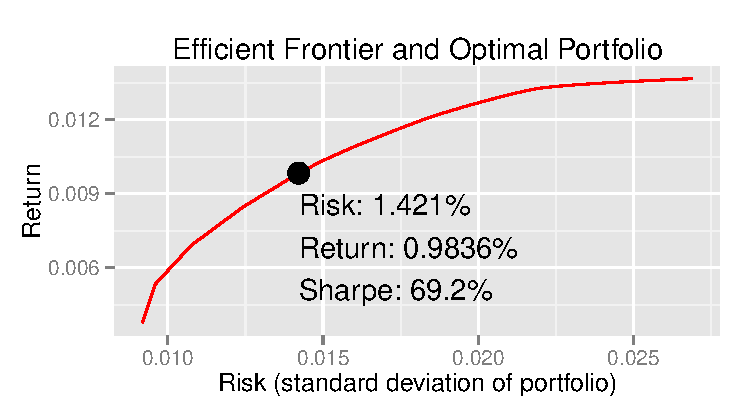
\includegraphics[width=\maxwidth]{figure/frontier-1} 

\end{knitrout}
    \caption{Efficient portfolio frontier and optimal allocation point.}
    \label{fig:frontier}
\end{figure}

\subsection{Bayesian Inference with Multinormal Distribution}

Unless otherwise noted, all of the Bayesian forms of the multivariate normal distribution come from Gelman \textit{et. al.} (2013).\cite{gelman13}. I will implement three versions of the Bayesian multivariate normal model. First, let's define the multivariate normal distribution as follows:

\begin{flalign}
    \mathbf{y}|\mathbf{\mu},\mathbf{\Sigma} \sim N(\mathbf{\mu},\mathbf{\Sigma})
\end{flalign}

As mentioned above, this is the simulation distribution of our asset returns. This model has the parameter vector of means $\mathbf{\mu}$ of length $d$ and the parameter matrix of variances and covariances $\mathbf{\Sigma}$ is $d$ by $d$. The probability density function of this model is

\begin{flalign}
    p(\mathbf{y}|\mathbf{\mu},\mathbf{\Sigma}) \propto |\mathbf{\Sigma}|^{-1/2} \exp \left(- \frac{1}{2} \left( \mathbf{y} - \mathbf{\mu} \right)^T \mathbf{\Sigma}^{-1} \left( \mathbf{y} - \mathbf{\mu} \right)  \right)
\end{flalign}

For $n$ independently and identically distributed (i.i.d.) observations, the likelihood is 

\begin{flalign}
    p(\mathbf{y}_1, \dots, \mathbf{y}_n |\mathbf{\mu},\mathbf{\Sigma}) \propto |\mathbf{\Sigma}|^{-n/2} \exp \left(- \frac{1}{2} \textrm{tr} \left( \mathbf{\Sigma}^{-1} \mathbf{S}_0 \right)  \right)    
\end{flalign}

$\mathbf{S}_0$ is the sum of squares matrix relative to $\mathbf{\mu}$ and is defined thusly,

\begin{flalign}
    \mathbf{S}_0 = \sum_{i=1}^{n}(\mathbf{y}_i - \mathbf{\mu})(\mathbf{y}_i - \mathbf{\mu})^T
    \label{}
\end{flalign}

When variance is known, the \textit{posterior distribution for $\mu$ with known $\mathbf{\Sigma}$} is as follows,

\begin{flalign}
    p(\mathbf{\mu}| \mathbf{y} \mathbf{\Sigma}) & \propto \exp \left( -\frac{1}{2} \left( \mathbf{\mu} - \mathbf{\mu}_n \right)^T \mathbf{\Lambda}_n^{-1} \left( \mathbf{\mu} - \mathbf{\mu}_n \right) \right) \notag \\
    & = N(\mathbf{\mu} | \mathbf{\mu}_n, \mathbf{\Lambda}_n)
    \label{}
\end{flalign}

The precision matrix $\mathbf{\Lambda}$ is the inverse of the covariance, and is easier to work with in certain distributions. I will define it and the parameterized version of $\mathbf{\mu}_n$ as follows,

\begin{flalign}
    \mathbf{\mu}_n & = \left( \mathbf{\Lambda}_0^{-1} + n \mathbf{\Sigma}^{-1} \right)^{-1} \left( \mathbf{\Lambda}_0^{-1} \mathbf{\mu}_0 + n \mathbf{\Sigma}^{-1} \bar{y} \right) \notag \\
    \mathbf{\Lambda}^{-1} & = \mathbf{\Lambda}_0^{-1} + n \mathbf{\Sigma}^{-1}
\end{flalign}

where $\mathbf{\mu}_0$ and $\mathbf{\Lambda}_0$ are the prior mean vector and variance matrix for the conjugate prior distribution of $\mathbf{\mu} \sim N(\mathbf{\mu}_0, \mathbf{\Lambda}_0)$. $\mathbf{\Sigma}$ is the sample variance and $\bar{y}$ is the sample mean.

For sampling purposes it is usually easier to work with the posterior conditional marginal distributions of subvectors of $\mathbf{\mu} $ with a known variance. Let the index $(-1)$ or $(-1,-1)$ indicate the absence of an element with the index $(1)$ or $(1,1)$ from the vector of means or matrix of variances. Then appropriate conditional and marginal distributions are,

\begin{flalign}
    \mu^{(1)}|\mathbf{\mu}^{(-1)}, \mathbf{y} \sim N\left( \mu_n^{(1)} + \beta^{1|2}\left( \mathbf{\mu}^{(-1)} - \mathbf{\mu}_n^{(-1)} \right), \mathbf{\Lambda}^{1|2} \right)
    \label{}
\end{flalign}

The regression coefficient $\beta^{1|2}$ and the conditional variance matrix $\mathbf{\Lambda}^{1|2}$ are defined as follows,

\begin{flalign}
    \beta^{1|2} & = \mathbf{\Lambda}_n^{(-1,1)} \left( \mathbf{\Lambda}_n^{(-1,-1)} \right)^{-1} \notag \\
    \mathbf{\Lambda}^{1|2} & = \mathbf{\Lambda}_n^{(1,1)} - \mathbf{\Lambda}_n^{(-1,1)} \left( \mathbf{\Lambda}_n^{(-1,-1)} \right)^{-1}  \mathbf{\Lambda}_n^{(1,-1)}
    \label{}
\end{flalign}

As it turns out, setting up the multivariate normal distribution with both an unknown mean and variance is even easier than when only the mean is unknown. The conjugate prior is parameterized as follows:

\begin{flalign}
    \mathbf{\Sigma} & \sim \textrm{ Inv-Wishart}_{v_0}\left( \mathbf{\Lambda}_0^{-1} \right) \notag \\
    \mathbf{\mu}|\mathbf{\Sigma}  & \sim N\left( \mu_0, \mathbf{\Sigma}/\kappa_0  \right)
    \label{}
\end{flalign}

The parameter $v_0$ is the number of degrees of freedom, and $\mathbf{\Lambda}_0$ is the scale matrix for the inverse-Wishart distribution.\footnote{Given a standard multivariate-normally distributed matrix $\mathbf{Z} \sim N(\mathbf{0}, \mathbf{\Sigma})$, a variable $\mathbf{W} = \mathbf{Z}^T \mathbf{Z}$ follows a Wishart distribution. In that sense, it is a multivariate generalization of the Chi-square distribution. If $\mathbf{W}$ follows a Wishart distribution, $\mathbf{S} = \mathbf{W}^{-1}$ follows the inverse Wishart distribution.} This is the final element we need in our algorithm create random matrices that follow multivariate normal distribution.

Using \texttt{R}, this distribution is available as a part of the \texttt{MCMC} package. In the distribution for the mean, $\kappa_0$ is the prior number of measurements used to calculate the mean.

From the prior density and the normal likelihood, we derive the following set of parameters.

\begin{flalign}
    \mathbf{\mu}_n & = \frac{\kappa_0}{\kappa_0 + n} \mu_0 + \frac{n}{k_0 + n} \bar{y} \notag \\
    \kappa_n & = \kappa_0 + n \notag \\
    v_n & = v_0 + n \notag \\
    \mathbf{\Lambda}_n & = \mathbf{\Lambda}_0 + \mathbf{S} + \frac{\kappa_0 n}{\kappa_0 + n} \left(\bar{y}  -\mu_0  \right) \left( \bar{y} -\mu_0 \right)^T
\end{flalign}

Sampling from this distribution occurs iteratively over two steps.

\begin{itemize}
    \item First, sample $\mathbf{\sigma}|\mathbf{y} \sim \textrm{ Inv-Wishart}_{v_n}\left( \mathbf{\Lambda}_n^{-1} \right)$
    \item Then, sample $\mathbf{\mu}|\mathbf{\Sigma},\mathbf{y}  \sim N\left( \mu_n, \mathbf{\Sigma}/\kappa_n  \right)$
\end{itemize}

If, instead, we want to employ a non-informative prior, the process only needs a few small adjustments.

\begin{itemize}
    \item First, sample $\mathbf{\sigma}|\mathbf{y} \sim \textrm{ Inv-Wishart}_{n-1}\left( \mathbf{S} \right)$
    \item Then sample $\mathbf{\mu}|\mathbf{\Sigma},\mathbf{y}  \sim N\left( \bar{y}, \mathbf{\Sigma}/n  \right)$
\end{itemize}

\subsection{Gibbs Sampling Algorithms}

A Gibbs sampler is a class of Markov Chain Monte Carlo (MCMC) that utilizes conditional probability distributions (German and German, 1984).\cite{german84} This is an important feature when we have distributions similar to the ones described above. In each of the three sampling cases, we will be working with marginal distributions that are conditioned on other parameters. In the case of the unknown variance, we condition on the other means. When the means and the variances are unknown, we condition the variance on the data and the mean on the variance.

In general, the Gibbs sampling algorithm is as follows. Suppose that $x$ is a vector of random variables, and $x = \left( x_1, \dots , x_d \right)$, and let $x_{[-A]}$ be ${x, j \in A^c}$ for any subset $A$ of the coordinates. The sample will ``update'' iteratively, so that at time $t+1$ you will have $x^{(t)} = \left( x_1^{(t)}, \dots , x_d^{(t)} \right)$.

\begin{itemize}
    \item For $i=1, \dots, d$, draw $x_i^{(t+1) }$ from the conditional distribution.

        \begin{flalign}
            \pi(x_i |x_1^{(t+1)}, \dots , x_{i-1}^{(t+1)}, x_{i+1}^{(t)} \dots x_d^{(t)})
        \end{flalign}

    \item The process updates along a chain. By the time it reaches $d$, all of the other elements will have been plugged in. For example,

        \begin{flalign}
            x_1^{(t+1)} & \sim \pi(x_1 | x_2^{(t)} \dots )   \notag \\
            x_2^{(t+1)} & \sim \pi(x_2 | x_1^{(t+1)}, x_3^{(t)} \dots) \notag \\
            x_3^{(t+1)} & \sim \pi(x_3 | x_1^{(t+1)}, x_2^{(t+1)}, x_4^{(t)} \dots )
        \end{flalign}

    \item Keep plugging in the conditional samples for each $i=1, \dots d$ until you get your sample.
\end{itemize}

All samples created with the Gibbs algorithm have 10,000 observations. Each was constructed using a burn-in period of 5,000 observations. This initial set of observations was thrown out to make sure that the algorithm had already converged.

\subsection{Validating Outcomes}

The same Monte Carlo techniques used to estimate the parameters for the Bayesian portfolios can also be used for validating the results. By simulating possible returns for each asset in the portfolio and the market as a whole, we can gain a sense of the frequency with which each individual portfolio will outperform the market. This is another performance dimension not fully captured by the Sharpe ratio.

While there is only market history to build our model on, alternative histories can be simulated. To do this, I calculated means and variances for the individual assets and the market index for 01-09-2012 to 12-30-2013. From there, 50,000 matrices consisting of 104 weeks of returns were simulated. With these new returns, I estimated the probabilities that our portfolio outperformed the market using a multivariate normal distribution. This is relatively easy, since you can just treat the variables like bivariate normals.

\begin{flalign}
P(X > Y) & = P (Y - X < 0) \notag \\
W & = Y - X \notag \\
W & \sim N(\mu_Y - \mu_X, \sigma_Y^2 + \sigma_X^2 - 2 \sigma_X \sigma_Y)
\end{flalign}

Using these simulated results, we can also assess the individual asset contribution to the total return. A well-designed and robust portfolio should generate returns across many different assets over an extended period. Otherwise, a particular portfolio outcome may have more to do with a particular market outcome than with our asset allocation. Given an $m$ by $n$ matrix of returns $\mathbf{X}$, where $m$ equals the periods in the simulation and $n$ is the number of assets, the vector of asset contributions $\mathbf{C}$ can be calculated as follows.

\begin{flalign}
  \mathbf{C} & = \frac{1}{\mu_p} \mathrm{D}(\mathbf{\omega_p}) \mathbf{X}^T \mathbf{1}_n
\end{flalign}

In the preceding formula, $\mu_p$ is the total return for a given portfolio, and $\mathrm{D}(\mathbf{\omega_p})$ is a diagonal matrix constructed from the corresponding asset weights. Ultimately, this amounts to the weighted column sums divided by their sum, i.e. a relatively simple proportion, which is calculated for each portfolio.

For the sake of interpretation, I index returns at 1 in this paper when discussing portfolio performance over a given period. In other words, all time series start at one instead of zero. But for these calculations, this indexing needs to be removed. If contribution for each asset is a portion of the total return, indexing at one will bias all of these ratios.

Last but not least, this contribution can be found for each simulation, which we can average for the final analysis. Moreover, we can find the stability of these contributions by looking at their variance. Under normal market conditions, we'd like to see somewhat evenly divided positive contributions with low variance for each asset. 

In particular, extremely large negative contributions indicate a misallocation. While small losses might occur from hedging within a diversified portfolio, large losses on certain assets in favor of massive returns on other assets is the equivalent leveraging. This strategy is risky and runs against the intuition of diversification. In fact this is the opposite. The analyst is making a large bet that only a portion of her chosen assets will perform well. She is putting all of her eggs in one basket.

\section{A Motivating Example}

\begin{figure}[H]
    \centering
\begin{knitrout}
\definecolor{shadecolor}{rgb}{0.969, 0.969, 0.969}\color{fgcolor}
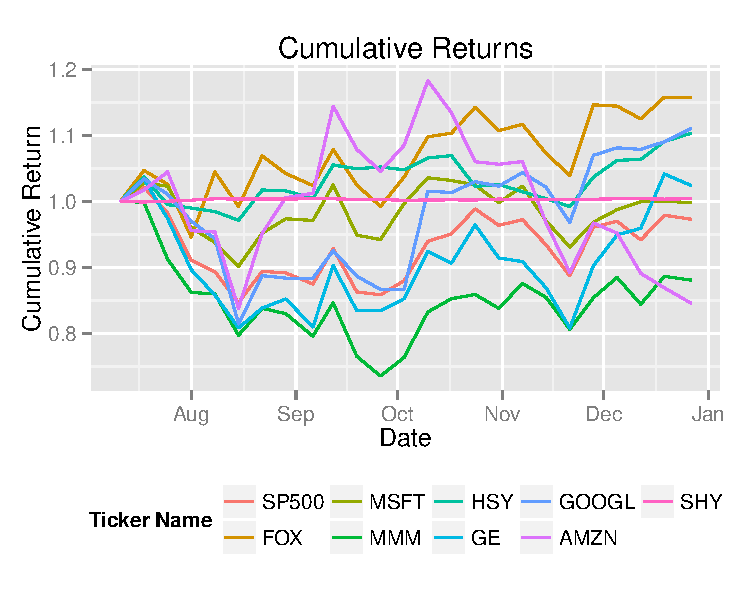
\includegraphics[width=\maxwidth]{figure/sixmonth-1} 

\end{knitrout}
    \caption{Indexed stock returns for the period of 07-18-2011 to 12-27-2011.}
    \label{fig:sixmonth}
\end{figure}

Consider the case of a hypothetical financial analyst at the end of 2011. The last year has been pretty rough, especially the last six months. High volatility in the market was matched with low returns, and many fund managers perform poorly in this sort of environment. See Figure~\ref{fig:sixmonth}. Nonetheless, with the beginning of the new year, there is broad consensus in future stock growth. This turns out to be correct, as the last few years have witnessed one of the strongest bull markets in recent history.

Our analyst downloads the previous year's weekly return data from \textit{Yahoo Finance} using the \texttt{stockPortfolio} package in \texttt{R}. She also has access on stock prices for most publicly traded assets dating back as far as 10 years. She believes that while the \textit{Yahoo Finance} data are more relevant to current market conditions, the older stock performance reports might minimize noise and has a better sense of ``long-term'' trends for these companies.

Given this environment, our analyst would like to build a new portfolio consisting of the following assets:

\begin{itemize}
    \item \texttt{FOX}: 21st Century Fox, Inc., the media holding company that includes stakes in film, television and satellite companies. It was formed during the Newscorp split, but has a ticker tape dating back to 1996.
    \item \texttt{MSFT}: Microsoft Corporation, the technology and consumer goods company.
    \item \texttt{MMM}: The 3M Company, a conglomerate that produces a wide array of consumer goods.
    \item \texttt{HSY}: The Hershey Company, a producer of candies and other foods.
    \item \texttt{GE}: General Electric, the multinational conglomerate which operates in the energy, technology, finance, consumer and industrial sectors.
    \item \texttt{GOOGL}: Google, the internet search engine and technology company.
    \item \texttt{AMZN}: Amazon.com, Inc., the online retailer.
    \item \texttt{SHY}: iShares Barclay's 1-3 Treasury Bond Fund, a proxy for a risk-free asset.
\end{itemize}

The performance of each of these assets is summarized in Table~\ref{tab:returns}, which shows annualized mean returns and annualized standard deviations. It also shows each asset's annualized Sharpe Ratio. The relatively high frequency of Sharpe ratios with a value less than one indicates difficult market conditions. It also tends to be a sign of market turbulence when the risk-free asset has the highest Sharpe ratio. 

\begin{table}
    \centering
    \resizebox{\columnwidth}{!}{%
\begin{tabular}{lrrrrrrrr}
  \hline
 & FOX & MSFT & MMM & HSY & GE & GOOGL & AMZN & SHY \\ 
  \hline
Annualized Return & 34.03 & -0.48 & -25.81 & 22.45 & 5.25 & 23.97 & -33.45 & 0.93 \\ 
  Annualized St. Dev. & 36.54 & 26.21 & 31.37 & 17.94 & 38.61 & 38.78 & 48.46 & 0.55 \\ 
  Sharpe Ratio & 0.93 & -0.02 & -0.82 & 1.25 & 0.14 & 0.62 & -0.69 & 1.70 \\ 
   \hline
\end{tabular} %
    }
\caption{Expected returns, standard deviations and Sharpe ratios for the candidate assets for the various portfolios to be shown below.}
    \label{tab:returns}
\end{table}

Our analyst believes that this is a somewhat representative portfolio for the American economy as a whole, providing a good opportunity for diversification. But it's also worth acknowledging that even this selection of assets is significantly smaller than an index like the \texttt{S\&P 500} or the \texttt{Dow Jones Industrial Average}. She will use the former as a benchmark for portfolio performance.

Using these data, she builds a naive Markowitz portfolio. She only uses the previous six months' means and variances. Unfortunately, this portfolio performs terribly over the next two years. The previous six months hardly resembled the emerging bull market.\footnote{Based on weekly returns from 01-09-2012 to 12-30-2013.} The analyst's basic portfolio had an annualized return of only 7.45\%, and an annualized standard deviation of 15.72\%. On the other hand the market (as shown by the returns to the \texttt{S\&P 500}) had an annualized return of 19.08\% and an annualized standard deviation of only 10.93\%. The market's Sharpe ratio was more than three times that of the analyst's portfolio (see Table~\ref{tab:results}).

While this is discouraging, it does not necessarily discredit the theory. Let's pose a counterfactual. What if the analyst had perfect foresight and could predict each asset's mean and variance over the next two years? With these impossible advantages, the Markowitz model performs dramatically better. It significantly reduces portfolio risk, and only slightly under-performs the market in absolute terms. This ``perfect foresight'' portfolio has a Sharpe ratio 271.11\%. This is obviously a sharp departure from reality, but it does provide a road towards improving the performance of the portfolio. 

Returning to the original formulation of the problem, the analyst has two pieces of information that are not incorporated into the basic estimates of parameters for the Markowitz model. There is general consensus that the market is due to improve, and the analyst has extensive historical data to provide context for recent returns. Her Bayesian prior, in the most general sense, is a composite of these two pieces of information. This is not perfectly useful, but it should be considered when constructing her portfolio. It certainly has the potential to improve over the basic portfolio's poor performance.

\section{Results}

Ultimately, improving portfolio performance comes down to improving estimates of parameters. Three scenarios are considered: only the mean is unknown, both parameters are unknown but the prior distribution is not informative, and the prior is informative.

Even under the noninformative conditions, I included an upward adjustment in means of 20\% for the priors. This is meant to capture the general consensus that market conditions will improve over the next two years. While space doesn't allow for validating the prior,\footnote{It's also not realistic. In practice the priors are set before developing the statistical model. If the results are poor, you simply set a better informed prior next time. We can't repeat history.} the Appendix demonstrates some simulations of returns using each of the portfolios. 

The annualized expected returns, standard deviations and Sharpe ratios for each of the portfolios in the project are included in Table~\ref{tab:results}. These results are found by applying the weights shown in Table~\ref{tab:weights} to the asset returns from 01-09-2012 to 12-30-2013. The weights give a good indication of which model portfolios hew closely to the parameters derived from the six months' of data available to the analyst. This can be found by simply comparing asset allocations.

\subsection{Bayesian Portfolios}

\begin{table}
    \centering
\begin{tabular}{lrrrr}
  \hline
 & Expected Return & Risk & Sharpe Ratio \\ 
  \hline
Market & 19.08 & 10.93 & 174.60\\ 
  Basic & 7.45 & 15.72 & 47.40 \\ 
  Foresight & 15.67 & 5.78 & 271.11 \\ 
  Unknown Mean & 8.50 & 13.76 & 61.76 \\ 
  Noninformative Prior & 7.46 & 15.66 & 47.62 \\ 
  Informative Prior & 32.10 & 14.04 & 228.65 \\ 
   \hline
\end{tabular}
    \caption{Annualized portfolio return and risk profiles for each of the estimation methods considered. The final three portfolios use Bayesian estimates.}
    \label{tab:results}
\end{table}

\begin{table}
    \centering
        \resizebox{\columnwidth}{!}{%
\begin{tabular}{lrrrrrrrr}
  \hline
 & FOX & MSFT & MMM & HSY & GE & GOOGL & AMZN & SHY \\ 
  \hline
Baseline & 25.12 & 45.08 & -50.00 & 50.00 & -12.09 & 27.90 & -36.01 & 50.00 \\ 
  Foresight & 11.40 & 0.89 & 19.39 & 16.76 & -2.91 & 3.88 & 0.59 & 50.00 \\ 
  Unknown Mean & 19.48 & 39.83 & -37.24 & 46.95 & -15.75 & 26.08 & -29.36 & 50.00 \\ 
  Noninformative Prior & 24.93 & 45.20 & -50.00 & 50.00 & -11.92 & 27.44 & -35.65 & 50.00 \\ 
  Informative Prior & 14.81 & 11.19 & 13.11 & 5.93 & 15.24 & 17.47 & 22.26 & -0.02 \\ 
   \hline
\end{tabular}%
    }
    \caption{Asset allocations for each of the portfolios in this project. The final three portfolios use Bayesian methods.}
    \label{tab:weights}
\end{table}

From the very beginning, we can get a sense of the factors contributing to the different performances of the basic and insight models. The latter has one asset that suffers from an extreme allocation, while the baseline model has three in addition to another model that is quite close to the limit. Financial theory generally predicts that portfolio performance improves with diversification, all other things being equal. Avoiding extreme allocations would be a plus.

As an alternative model, the first Bayesian portfolio was generated using an unknown mean but a known variance. From the analyst's perspective, this is akin to the assumption that while returns over the last six month were clearly not representative, overall market variation was not extremely atypical. This attitude is supported in the literature, which notes that mean estimates have a much stronger effect on the Markowitz model than variance estimates.

Following the model set out by Gelman, \cite{gelman13} the unknown mean model returns a parameter that is hardly distinguishable from that of the basic Markowitz model. This is a good thing in most circumstances, but not a particular benefit here. Rachev suggests solving this issue by readjusting weights on the prior and the data based on investor confidence. \cite{rachev08} Since other estimation options are available here, I just moved on.

\begin{figure}[t]
    \centering
\begin{knitrout}
\definecolor{shadecolor}{rgb}{0.969, 0.969, 0.969}\color{fgcolor}
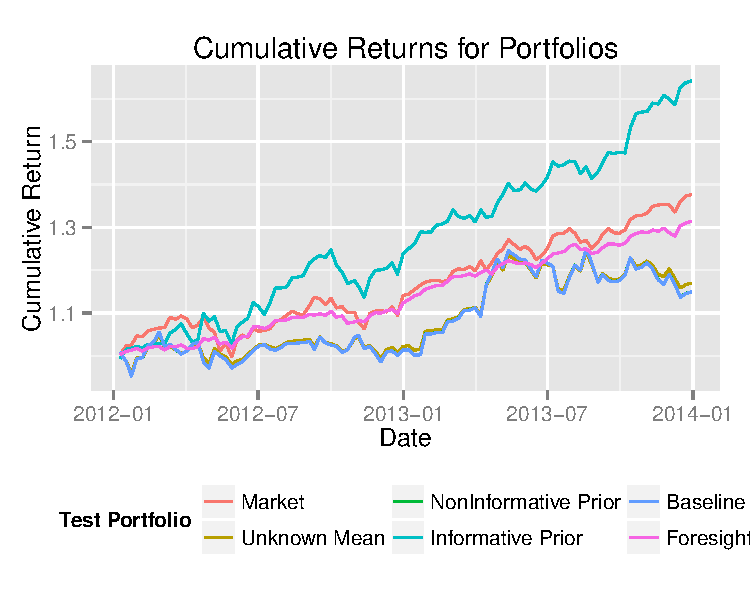
\includegraphics[width=\maxwidth]{figure/results-1} 

\end{knitrout}
    \caption{Cumulative returns for each model portfolio, as tested against asset data from 01-09-2012 to 12-30-2013.}
    \label{fig:cumret}
\end{figure}

The same issues appeared with the model relying on a noninformative prior. Once again, this should be expected given the mathematical and theoretical basis of noninformative priors, but this is not the desired result. Moreover, little can be done to add a subjective ``correction'' to the model or gain any benefit from general knowledge. Strictly speaking, that is the point of a noninformative prior. 

On the other hand, real improvements are achieved by applying analysts' prediction of growth and the full weight of preexisting knowledge through the long-term asset means and variances. Furthermore, we can diminish the problematic effects of recent data by weighting the model parameters using the much larger number of observations in these historical estimates.

While the final Bayesian model still does not outperform the foresight portfolio in terms of Sharpe ratio, it has a much higher return. In fact, it is the only portfolio that outperforms the market index in absolute terms. The performance is achieved by acquiring much higher risk, an appropriate response during a period of high returns. Nonetheless, this portfolio retains a much higher Sharpe ratio than market. Either way, this portfolio is better.

The gains in performance come through avoiding extreme allocations while favoring generally risky assets over the safer risk-free asset. In fact, this is the only portfolio that does not take the maximum allocation possible for the risk-free asset. Although the risk-free asset had the highest Sharpe ratio during the six months of data available to the analyst, this is not the general case. It certainly wasn't true for the following two years (see Table~\ref{tab:test}), and it is not sound financial thinking to favor risk-free assets during bull markets.

\begin{table}
    \centering
        \resizebox{\columnwidth}{!}{%
\begin{tabular}{lrrrrrrrr}
  \hline
 & FOX & MSFT & MMM & HSY & GE & GOOGL & AMZN & SHY \\ 
  \hline
Annualized Return & 0.40 & 0.20 & 0.29 & 0.27 & 0.25 & 0.30 & 0.43 & 0.00 \\ 
  Annualized St. Dev. & 0.18 & 0.22 & 0.13 & 0.13 & 0.17 & 0.22 & 0.28 & 0.00 \\ 
  Sharpe Ratio & 2.19 & 0.88 & 2.22 & 1.99 & 1.52 & 1.32 & 1.55 & 0.59 \\ 
   \hline
\end{tabular}%
    }
    \caption{Expected returns, standard deviations and Sharpe ratios for the candidate assets for the various portfolios over the test period. The data used for estimating these statistics cover 01-09-2012 to 12-30-2013.}
    \label{tab:test}
\end{table}

\subsection{Validation}

Sharpe ratios are a useful tool for assessing overall performance, but they aren't the only tool available. When looking at these ratios, it's worthwhile to keep in mind that a single market outcome is not generalizable and previous market performance is not a guarantee for future performance. More intuitively, this is an issue of simulation. We can't observe more than one stock market, but we can at least generate possible market outcomes given a set of parameters.

\begin{table}
    \centering
\begin{tabular}{lrrr}
  \hline
 & Return & St. Dev. & P $>$ Market \\ 
  \hline
Baseline & 1.15 & 0.22 & 0.19 \\ 
  Insight & 1.31 & 0.08 & 0.26 \\ 
  Unknown Mean & 1.17 & 0.20 & 0.19 \\ 
  Noninformative Prior & 1.15 & 0.22 & 0.19 \\ 
  Informative Prior & 1.64 & 0.20 & 0.99 \\ 
  Market & 1.38 & 0.16 & 0.00 \\ 
   \hline
\end{tabular}
    \caption{Starting from the left, the total expected return after two years in the simulation indexed with $t_0 = 1$. The is followed by the standard deviation of these total returns and the probability that the portfolio will outperform the market after two years. This probability assumes return normality and depends on the means and standard deviations in the table.}
    \label{tab:simulations}
\end{table}

If the underlying assumptions given the normality of the returns is correct, the informative prior will outperform the market 98.93\% of the time over this investment horizon. This is much better than the probability of the portfolio with foresight beating the market. That said, the much higher returns of the informative prior come through the willingness to accept more risk.

We can visualize these relationships with a series of plots. Overlays of the distributions are nice in that they allow for easy comparisons of the portfolio and the market. In particular, since the distributions are all roughly normal, overlays allow for easy comparisons of center and spread. On the other hand, the overlays cannot give a sense of the correlation between the two distributions and the final calculation of inequalities within the probability statements. See Figure~\ref{fig:probsinform} for the distribution plots for the Bayesian portfolio with an informative prior.

\begin{figure}[H]
\begin{knitrout}
\definecolor{shadecolor}{rgb}{0.969, 0.969, 0.969}\color{fgcolor}
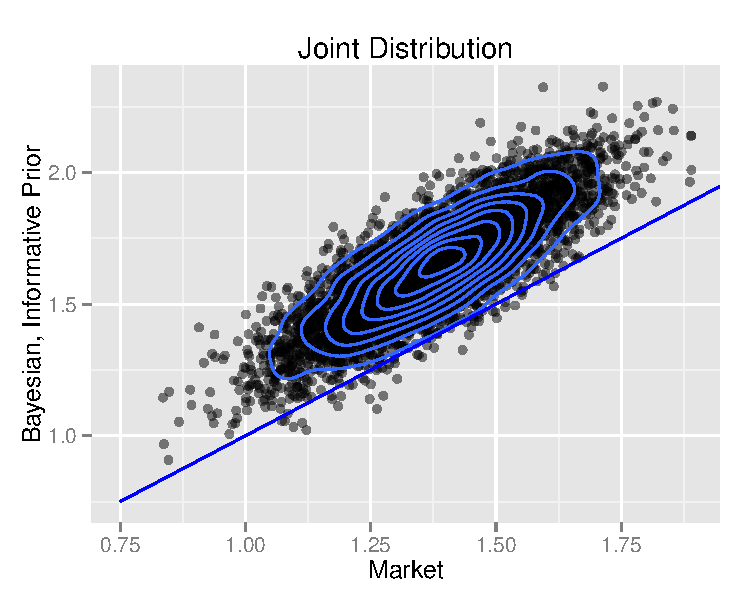
\includegraphics[width=.49\linewidth]{figure/dist-pair-inform-1} 
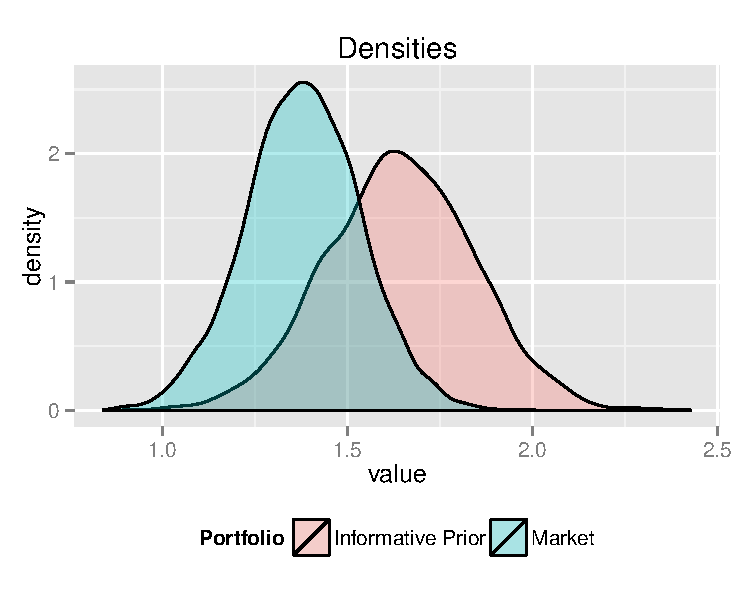
\includegraphics[width=.49\linewidth]{figure/dist-pair-inform-2} 

\end{knitrout}
\caption{On the left: A joint density plot for the market index and the Bayesian portfolio with an informative prior. Contour lines and annotation for where $Y > X$ are included. On the right: An overlay of the two densities.}
\label{fig:probsinform}
\end{figure}

One question remains about these results: What drives this improved performance? If we're interested in generalizability, it would be worrisome if these results came through the performance of only a single asset. To be blunt, it would be the result of luck, not improved analytic techniques.

\begin{table}[ht]
\centering
\resizebox{\columnwidth}{!}{%
\begin{tabular}{lrrrrrrrr}
  \hline
 & AMZN & FOX & GE & GOOGL & HSY & MMM & MSFT & SHY \\ 
  \hline
Baseline & 8.96 & -2.79 & 1.16 & -2.80 & -4.24 & 4.56 & -3.82 & -0.02 \\ 
  Foresightsight & 0.02 & 0.29 & -0.05 & 0.07 & 0.28 & 0.36 & 0.01 & 0.01 \\ 
  Unkown Mean & 0.49 & -0.26 & 0.37 & -0.11 & 0.29 & 0.53 & -0.29 & -0.01 \\ 
  Noninformative Prior & 0.12 & -0.47 & 0.13 & 0.15 & -0.47 & 0.80 & 0.76 & -0.01 \\ 
  Informative Prior & 0.29 & 0.19 & 0.12 & 0.16 & 0.05 & 0.12 & 0.07 & -0.00 \\ 
   \hline
\end{tabular}%
    }
    \caption{Mean asset contributions to 5,000 simulated portfolio returns for the five portfolios examined in this project. The final three rows refer to portfolios constructed using Bayesian estimates of the parameters.}
    \label{tab:contmeans}
\end{table}

\begin{table}[h]
\centering
\resizebox{\columnwidth}{!}{%
\begin{tabular}{lrrrrrrrr}
  \hline
 & AMZN & FOX & GE & GOOGL & HSY & MMM & MSFT & SHY \\ 
  \hline
Baseline & 720.01 & 228.97 & 87.10 & 264.76 & 360.50 & 368.80 & 318.29 & 1.37 \\ 
  Foresight & 0.01 & 0.07 & 0.02 & 0.04 & 0.08 & 0.08 & 0.01 & 0.01 \\ 
Unkown Mean & 100.23 & 52.99 & 36.11 & 51.27 & 89.71 & 102.23 & 53.32 & 2.21 \\ 
Noninformative Prior & 146.76 & 82.96 & 27.74 & 57.01 & 86.63 & 119.31 & 77.86 & 0.93 \\ 
Informative Prior & 0.40 & 0.18 & 0.10 & 0.18 & 0.12 & 0.11 & 0.14 & 0.00 \\ 
   \hline
\end{tabular}%
    }
    \caption{Standard deviation of asset contributions to 5,000 simulated portfolio returns for the five portfolios examined in this project. The final three rows refer to portfolios constructed using Bayesian estimates of the parameters.}
    \label{tab:contsds}
\end{table}

Looking at contributions and contribution standard deviations (see Tables~~\ref{tab:contmeans} and~\ref{tab:contsds}), we can see that the foresight and informative prior portfolios show similar results, with evenly distributed contributions among the chosen assets and relatively low variances. The same cannot be said about the other portfolios. The baseline portfolio, in particular, derives the overwhelming majority of its total return from the performance of a single asset. This is not a prudent decision.

Looking at the asset contributions to total portfolio returns, the portfolio based on the informative prior outperforms the insight portfolio by generating wealth across all assets in the portfolio while avoiding losses. At the same time, variances in contributions indicate a degree of risk similar to higher variances in asset returns. The low variances in asset returns in the insight portfolio indicates that returns remain consist, and are derived in similar amounts from similar sources, across a range of market conditions.

\section{Conclusions}

While the results are encouraging, we should resist the temptation to read too much into them. First, drawing general conclusions from a single period of stock market performance is difficult. Even when we try to resample returns to make outcomes more general (as occurred in the preceding validations), it is difficult to believe that any one period of returns will resemble another. Moreover, with the work provided above, it is also hard to find a suitable balance between the different pieces of information going into the model. The use of an informative seems to indicate that the portfolio will do better when it is weighted away from the data of the previous three months. But how much is appropriate? At this point, it's still hard to say.

With those things in mind, these small experiments highlight some positive features. For one, a Bayesian framework of parameter estimation allows the analyst to incorporate a broader spectrum of information. No doubt, this is beneficial and important in a setting like the stock market. A lot of useful information about stock prices is available and waiting tools for incorporating it into pricing models and portfolio design. Moreover, as Rachev shows, \cite{rachev04} a variety of models can be balanced using a similar Bayesian framework. 

Bayesian methodologies would be useful to financial analysts in Kazakhstan, as it is a data-poor country. Kazakhstan does not differ from other developing countries in that regard. The Kazakhstan Stock Exchange (KASE) provides information to institutional investors, but it pales in comparison to the data available in Western markets. Furthermore, locally generated financial and economic data are often perceived as unreliable. Whether this is warranted or not is a separate discussion. Combined these factors pose a risk to all Kazakhstani investors.

What can be done? The institutions needed for better financial data might not be developed for a long time, but there is a large amount of information available from local experts, businessmen and politicians. A Bayesian analyst would seize the opportunity to incorporate this information through informative priors. As Kazakhstan has experienced several periods of high volatility and uncertainty, like the example given in this paper, informative priors have the potential to improve the performance of portfolios. 

For people familiar with work in business in Kazakhstan, these recommendations may seem like common sense. Most would agree that personal connections and word-of-mouth channels are critical to understanding the local business climate. Nonetheless, these heuristics often lack a reliable rigorous framework, as is the case with ad hoc techniques for building portfolios. In that regard, Bayesian methodologies encourage a broader selection of knowledge along with robust mathematical techniques.


\begin{thebibliography}{99}
        \bibitem{best91} Best, M. J., \& Grauer, R. R. (1991). On the sensitivity of mean-variance-efficient portfolios to changes in asset means: some analytical and computational results. \textit{Review of Financial Studies}, 4(2), 315-342.
        \bibitem{black92} Black, F., \& Litterman, R. (1992). Global portfolio optimization. Financial \textit{Analysts Journal}, 28-43.
        \bibitem{clement99} Clement, M. B. (1999). Analyst forecast accuracy: Do ability, resources, and portfolio complexity matter?.\textit{ Journal of Accounting and Economics}, 27(3), 285-303.
        \bibitem{chopra93} Chopra, V. K., \& Ziemba, W. T. (1993). The effect of errors in means, variances, and covariances on optimal portfolio choice. \textit{The journal of portfolio management}, 19(2), 6-11.
        \bibitem{const95} Constantinides, G. M., \& Malliaris, A. G. (1995). Portfolio theory. \emph{Handbooks in operations research and management science}, 9, 1-30.
        \bibitem{gelman13} Gelman, A., Carlin, J. B., Stern, H. S., Dunson, D. B., Vehtari, A., \& Rubin, D. B. (2013). \textit{Bayesian data analysis}. CRC press.
        \bibitem{german84} Geman, S., \& Geman, D. (1984). Stochastic relaxation, Gibbs distributions, and the Bayesian restoration of images.\textit{ Pattern Analysis and Machine Intelligence, IEEE Transactions on}, (6), 721-741.
        \bibitem{hoff09} Hoff, P. D. (2009). \textit{A first course in Bayesian statistical methods}. Springer Science \& Business Media.
        \bibitem{kruschke10} Kruschke, J. (2010). Doing Bayesian data analysis: A tutorial introduction with R. Academic Press.
        \bibitem{mandel04} Mandelbrot, B., \& Hudson, R. L. (2004). \textit{The (Mis)Behaviour of Markets: A Fractal View of Risk, Ruin, and Reward}. London: Profile Books.
        \bibitem{mark52} Markowitz, H. (1952). Portfolio selection*. \textit{The journal of finance}, 7(1), 77-91. 
    \bibitem{matu13} Matuszak, A. (2013). Building an Optimized Portfolio with R. \textit{Modern Portfolio Theory}. Retrieved on May 5, 2012 from \url{http://economistatlarge.com/portfolio-theory/r-optimized-portfolio}. 
       \bibitem{rachev04} Ortobelli, S., Rachev, S., Huber, I., \& Biglova, A. (2004). Optimal portfolio selection and Risk management: A comparison between the stable paretian approach and the Gaussian one. In \textit{Handbook of Computational and Numerical Methods in Finance (pp. 197-252)}. Birkhäuser Boston.
        \bibitem{rachev08} Rachev, S. T., Hsu, J. S., Bagasheva, B. S., \& Fabozzi, F. J. (2008). \textit{Bayesian methods in finance} (Vol. 153). John Wiley \& Sons.
        \bibitem{ruppert10} Ruppert, D. (2010). \textit{Statistics and data analysis for financial engineering}. Springer.
        \bibitem{zivot13} Zivot, E. (2013). Portfolio theory matrix algebra. Retrieved on May 5, 2012 from \url{http://faculty.washington.edu/ezivot/econ424/portfolioTheoryMatrix.pdf}.
\end{thebibliography}

\end{document}
